\exercisetitle{
En el circuito de la figura, usar la carta de Smith para encontrar el SWR de la línea, el coeficiente de reflexión en la carga, la admitancia de carga, la impedancia de entrada de la línea, la distancia desde la carga hasta el primer mínimo de voltaje, y la distancia desde la carga al primer máximo de voltaje.
}
Primero normalizaremos la impedancia en la carga como: $z_l = 1.4 + 0.8j$
\subsection{SWR y $\Gamma$}
Para calcular estos valores usando la carta de smith situamos la impedancia normalizada en la carta y medimos la distancia hasta el origen (0, 0),  usando las diferentes escalas en la parte de abajo podremos obtener los valores.
Estos valores resulta SWR = 2 y $\Gamma = 0.32$
\begin{figure}[h]
  \centering
  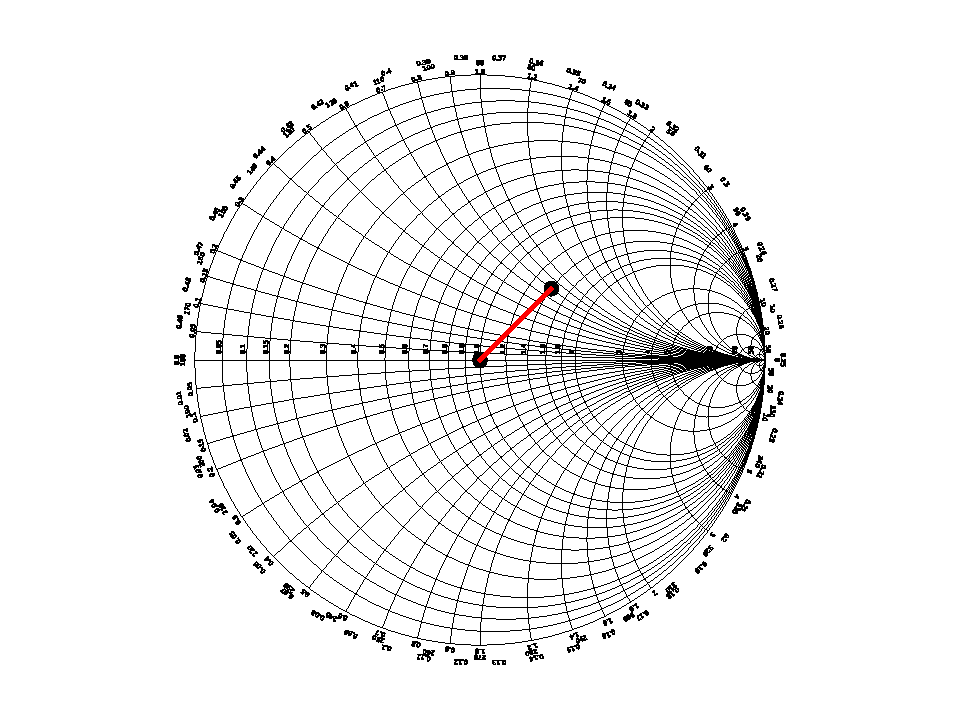
\includegraphics{ej7/images/out1.pdf}
  \caption{SWR y $\Gamma$}
  \label{ej2smith}
\end{figure}
\newpage
\subsection{Admitancia de la carga}
Para calcular la admitancia moveremos el punto anteriormente obtenido $180\º$ y denormalizaremos el mismo multiplicando por $\frac{1}{Y_0}$
\begin{figure}[h]
  \centering
  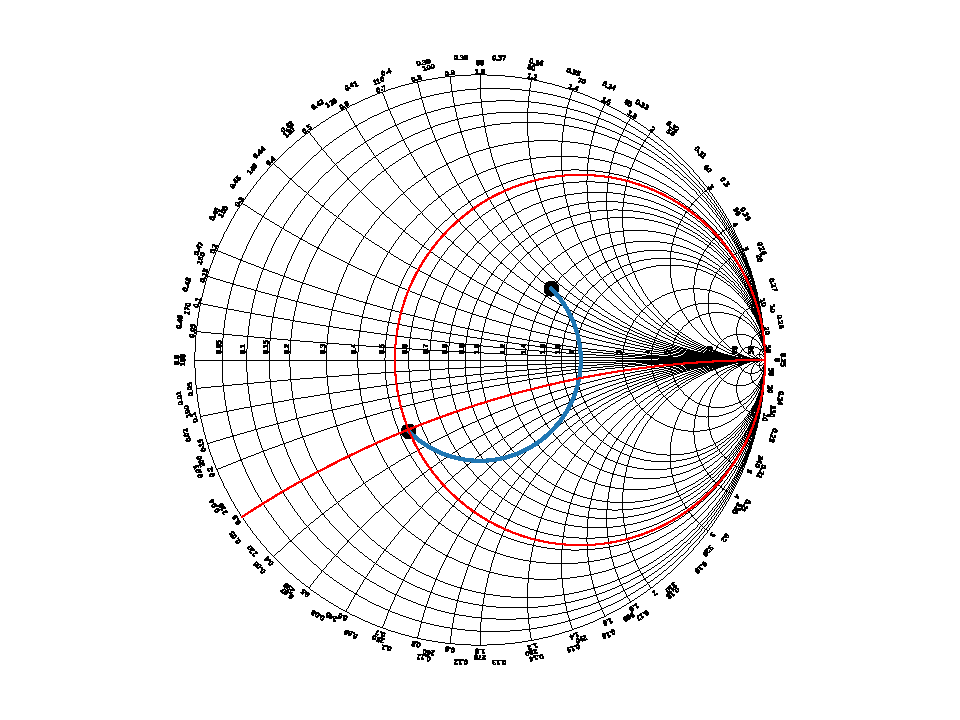
\includegraphics{ej7/images/out2.pdf}
  \caption{Admitancia}
  \label{ej2smith}
\end{figure}
\newline
Donde al denormalizar obtenemos $Y_l =  0.018 + j6 \times 10^{-3} S$
\newpage

\subsection{Impedancia de entrada}
Para hayar la impedancia de entrada simplemente moveremos el punto obtenido en primer apartado $0.8\lambda$ hacia el generado y denormalizaremos la impedancia

\begin{figure}[h]
  \centering
  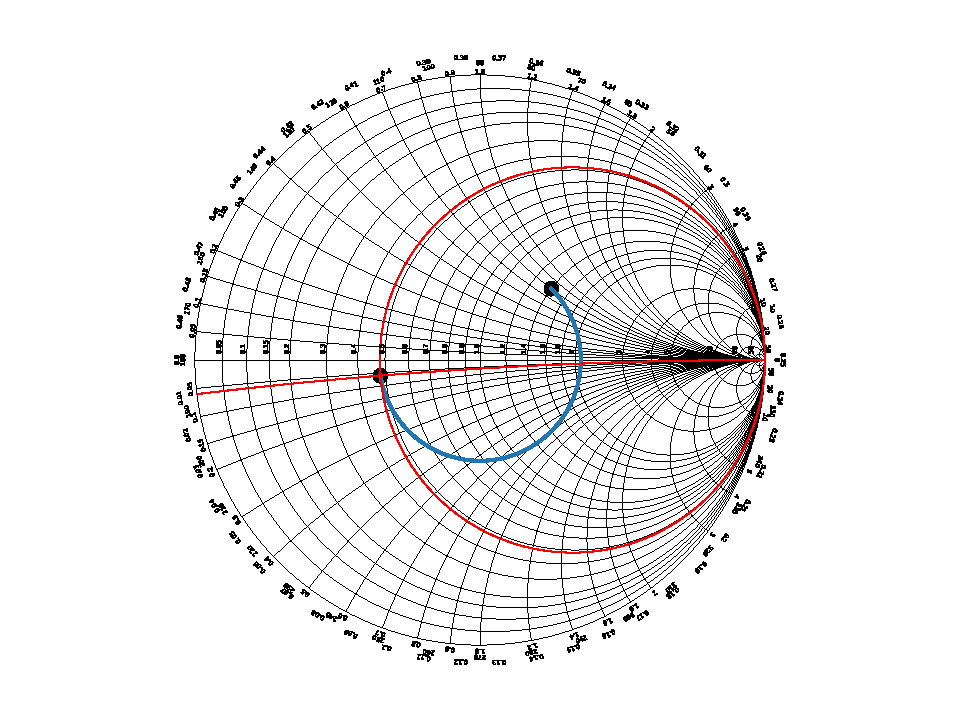
\includegraphics{ej7/images/out3.pdf}
  \caption{Impedancia de entrada}
  \label{ej2smith}
\end{figure}
Al denormalizar obtenemos $Z_{in} = 24 + 3j \Omega$
\newpage

\subsection{Máximo y mínimo}
Para hayar la distancia del primer máximo/mínimo nos fijaremos en el detalle de que los máximos y mínimos en la línea se producen cuando $Z(-l)$ es un número puramente real, por lo tanto la estrategia que seguiremos para hayar dichos puntos será avanzar el punto calculado en el apartado 1 hasta que la parte imaginaria sea 0, el siguiente máximo/minimo se encotrará a $\lambda / 4$ de este punto.
\begin{figure}[h]
  \centering
  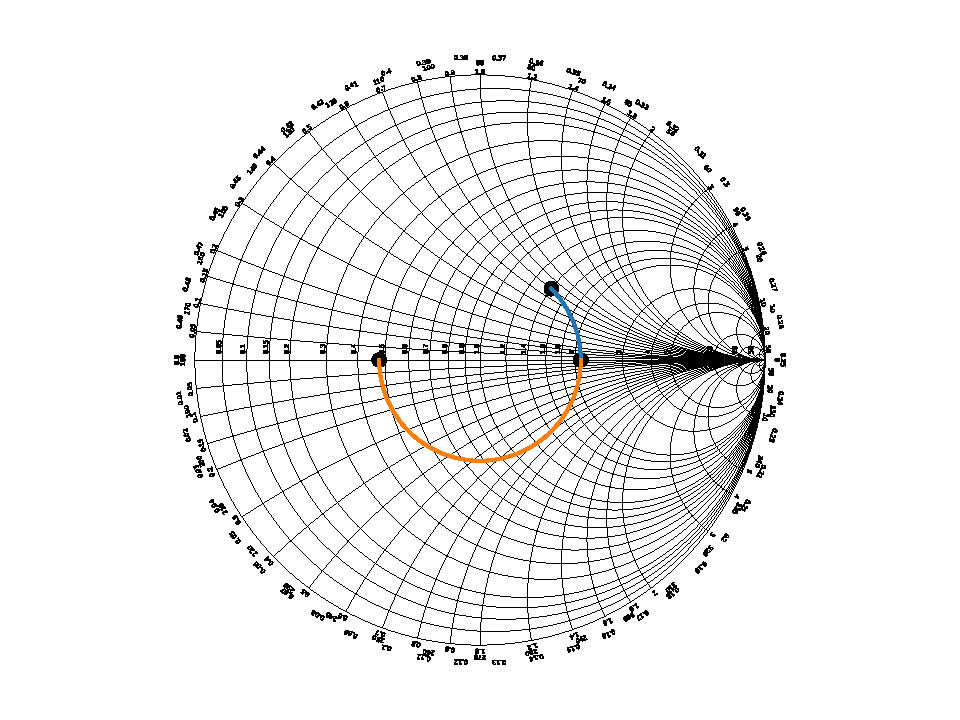
\includegraphics{ej7/images/out4.pdf}
  \caption{Máximo y mínimo}
  \label{ej2smith}
\end{figure}
Donde vemos que la distancia, en longitudes de onda, hasta el primer máximo ($Z_0 \leq Z(-l)$ ) es de $0.028\lambda$, por lo que el mínimo se encontrará a $0.278\lambda$.
